\documentclass{article}
\usepackage[utf8]{inputenc}
\usepackage{geometry}
\geometry{a4paper, top=2.5cm, bottom=2.5cm, left=3cm, right=3cm, bindingoffset=5mm}
\usepackage[table]{xcolor}
\usepackage{multirow}
\usepackage{colortbl}
 
\usepackage{multicol}
\usepackage{hyperref}
\usepackage{capt-of}
\usepackage{url}
\usepackage{graphicx}
\usepackage[italian]{babel}
\usepackage[suftesi]{frontespizio}


\title{Relazione di Laboratorio: Velocità della luce}

\author{Gruppo VE\_2:\\ \\Federico Greco C.M 969073\\federico.greco2@studenti.unimi.it\\ \\ Nicolò Favagrossa C.M. 969124\\nicolo.favagrossa@studenti.unimi.it\\ \\Daniele Hasou C.M. 967555\\daniele.hasou@studenti.unimi.it \\ \\ Esperimento eseguito da: Nicolò Favagrossa, Federico Greco e Daniele Hasou}
\date{\today\\A.A. 2021-2022}

\begin{document}
\maketitle
\newpage
\tableofcontents
\newpage
\section{Introduzione}
La misura della velocità della luce ha un interesse fisico molto elevato in quanto rappresenta uno dei valori notevoli con importantissime ripercussioni concrete nella realtà in cui viviamo. Uno dei primi tentativi concreti di misurare la velocità della luce è stato effettuato durante il XVI secolo da Galileo Galilei, che sospettava che la luce non si propagasse istantaneamente. Altri tentativi vennero svolti durante il XVII e XVIII secolo da Olaus Roamer attraverso osservazioni  astronomiche.\\

La difficoltà di questa misura risiede negli ordini di grandezza:  se si vuole misurare la velocità della luce a partire dalla formulazione classica (spazio percorso diviso al tempo necessario per percorrerlo) si incontrano svariati problemi originati dagli enormi spazi richiesti e dai piccolissimi tempi ottenuti. Per riuscire a misurare più agevolmente la velocità della luce serve dunque trovare un fenomeno alternativo che dipenda da tale grandezza ma che sia facilmente misurabile e non richieda apparati strumentali eccessivamente grandi. Così nel 1849, Hippolyte Fizeau sviluppò un nuovo metodo, successivamente modificato da Foucault.\\

Il metodo di Fizeau era basato su una ruota dentata, in grado di ruotare a velocità angolare decisa dallo sperimentatore, sul cui bordo veniva mandato un raggio luminoso (in modo che questo venisse bloccato o meno in presenza o assenza di un dente della ruota). Ponendo uno specchio piano distante dalla ruota, affinché il raggio venisse riflettuto e tornasse indietro percorrendo il medesimo tragitto dell'andata, ci si rende conto che l'intensità luminosa che ritorna al punto della sorgente è minima a velocità angolari della ruota ben precise, che corrispondono alle velocità angolare necessaria affinché un dente della ruota occupi lo spazio occupato da un buco nel tempo in cui la luce compie il percorso di andata e di ritorno. A partire da tali valori di velocità angolare, è possibile calcolare la velocità della luce.\\

Il problema legato al metodo di Fizeau deriva dal fatto che pur utilizzando un fascio di luce molto collimato come può essere la luce prodotta da un laser, a grande distanza (nell'ordine di $10\,km$) diverge. Un'altra complicazione consiste nel posizionare lo specchio in modo tale che sia perfettamente allineato e che faccia tornare il fascio di luce esattamente da dove è arrivato. o anche semplicemente dalla non omogeneità dello spazio percorso dalla luce in quanto può cambiare l'indice di rifrazione.
%Parola importante è collimare e sapere bene cosa è un collimatore (detto dalla prof a lezione)
Nel 1850 fu introdotto il metodo di Foucault, adottato in laboratorio, in cui viene completamente rimossa la ghiera rotante e vengono introdotti uno specchio concavo e uno specchio rotante.
\begin{figure}[htp!]
  \centering
  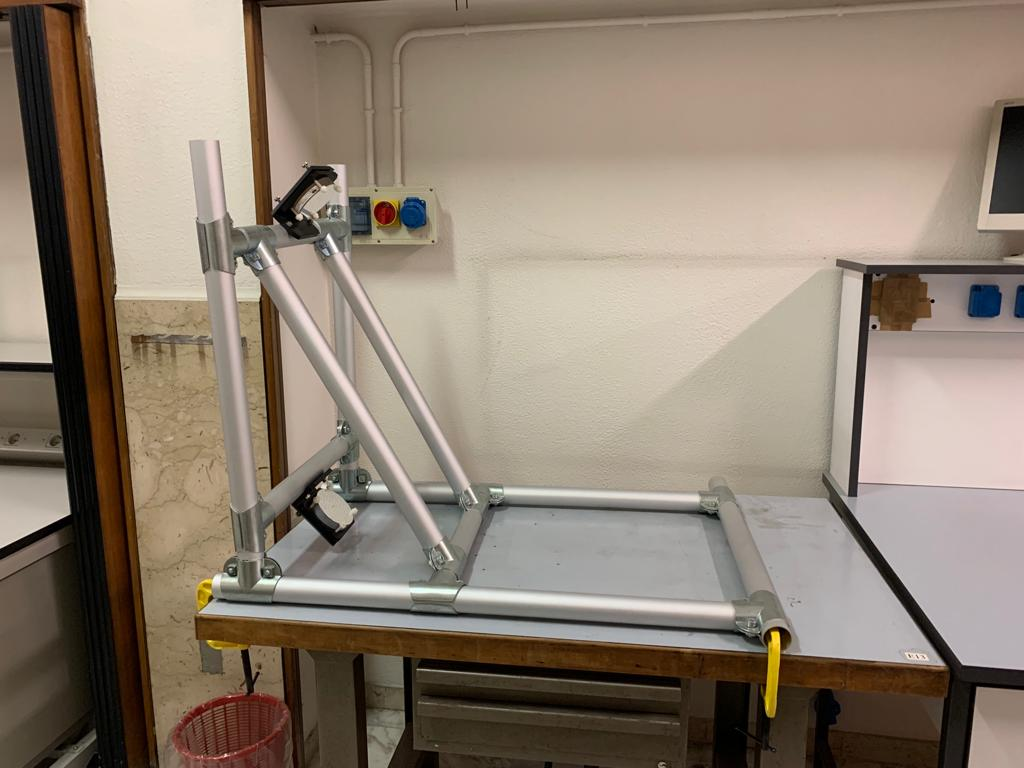
\includegraphics[scale=0.18]{Immagini/2.jpeg} 
  \centering
  \qquad 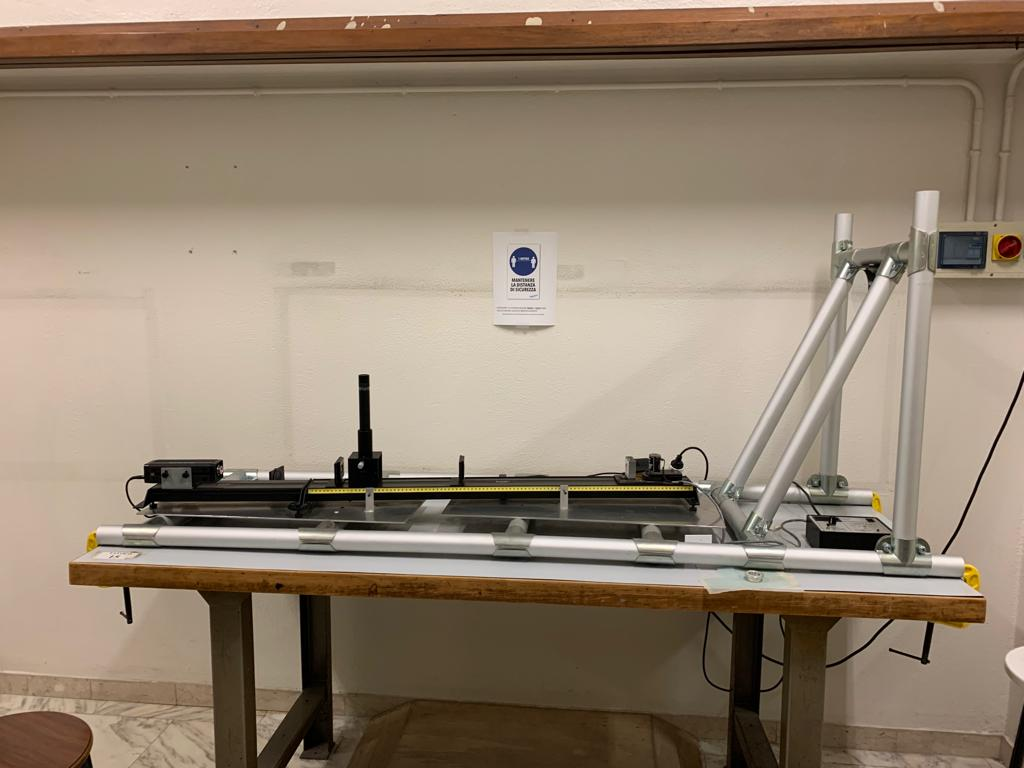
\includegraphics[scale=0.18]{Immagini/1.jpeg}
  \caption{Nelle due immagini si può osservare sistema sperimentale presente in laboratorio. Nella prima foto sono presenti i due specchi piani mentre a destra (posti ad una distanza considerevole) è presente l'apparato principale composto dal laser, ottiche, specchio concavo e rotante.}
\end{figure}
\newpage
\section{Trattazione teorica}
Una schematizzazione dell'apparato usato da Foucault è rappresentato nell'immagine (\ref{App}):\\

\noindent\begin{minipage}{0.5\textwidth}% adapt widths of minipages to your needs
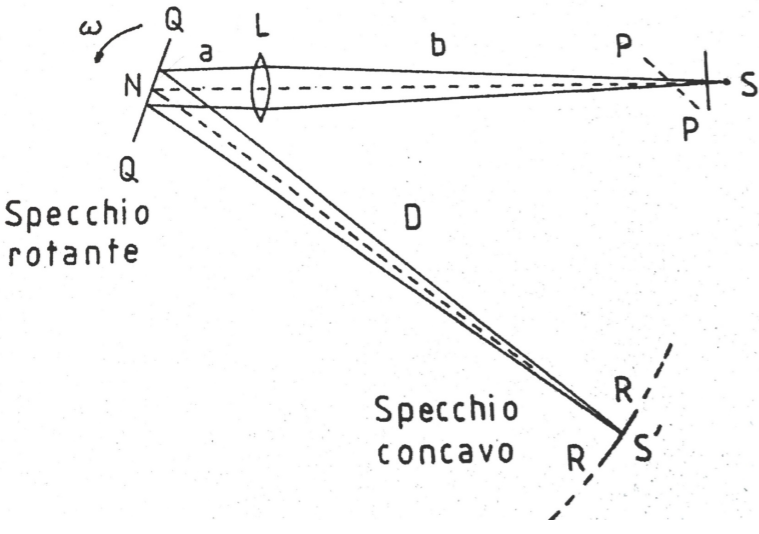
\includegraphics[width=\linewidth]{foucault2.png}
\end{minipage}%
\hfill%
\begin{minipage}{0.5\textwidth}\raggedleft
\begin{itemize}
    \item S è la sorgente luminosa, approssimata puntiforme, da cui parte il fascio luminoso;
    \item Q è uno specchio piano rotante;
    \item R è uno specchio sferico fisso;
    \item L è una lente convergente, tale da convergere il fascio luminoso proveniente da S sul centro dello specchio R;
    \item P è una lastra semitrasparente, necessaria per l'osservazione dei fenomeni
    \item b rappresenta la distanza tra P e L
    \item a rappresenta la distanza tra L e Q
    \item D rappresenta la distanza tra Q ed R
\end{itemize}
\end{minipage}\\



La sorgente luminosa S emette un fascio di luce che, dopo essere stato diaframmato, attraversa una superficie semitrasparente P inclinata di 45° rispetto alla direzione del fascio. Quest'ultimo successivamente attraversa una lente, che porta i raggi luminosi prima a riflettersi nello specchio rotante Q, poi a focalizzarsi sullo specchio concavo R nel punto S', ed infine tornare indietro.
Quando però lo specchio rotante Q viene messo in rotazione a velocità angolare $\omega$, si ha che l'immagine prodotta dalla sorgente S' non coincide più con il raggio di andata: nel tempo necessario affinché la luce compia la distanza D, lo specchio rotante avrà compiuto una rotazione di un angolo $\alpha$ dato da 
\begin{equation}
    \alpha=2(D/c)\omega,
\end{equation}
dove $c$ rappresenta appunto la velocità della luce nell'aria. Il fascio luminoso proveniente da S' viene focalizzato dalla lente L come se provenisse da una sorgente S'', spostata dal S' di una quantità che viene approssimata a 
\begin{equation}
    \Delta=2\alpha D
\end{equation}
essendo l'angolo $\alpha$ sufficientemente piccolo da permettere approssimazioni algebriche senza perdita di significatività.
Una volta attraversata la lente, il fascio luminoso subisce un ingrandimento di modulo pari a 
\begin{equation}
    G=b/(D+a),
\end{equation}
dove $b$ rappresenta la distanza tra la sorgente S e la lente e $a$ indica la distanza tra la lente L e il punto fisso N dello specchio rotante Q.
Sulla lastra semitrasparente P viene dunque uno spostamento $\delta$ pari a 
\begin{equation}
    \delta=G\Delta=\frac{4D^2b\omega}{c(D+a)}
    \label{delta}
\end{equation}

Un problema legato a questa esperienza è quello della luminosità dell'immagine prodotta: l'apparato produce un punto luminoso fintanto che il fascio riflesso dallo specchio rotante colpisce lo specchio concavo. Il rapporto tra la luminosità dell'immagine emessa dalla sorgente S e quella che ritorna sulla lastra semitrasparente P dipende fortemente dalle dimensioni dello specchio concavo e dalla sua apertura. Se la luminosità dell'immagine su P fosse troppo ridotta, non si potrebbe misurare la distanza $\Delta \delta$ e fallirebbe l'esperimento: per ovviare a questo problema, si può scegliere di utilizzare un produttore di raggi laser come sorgente S: l'altissima luminosità di tale raggio garantisce una discreta visibilità del fascio di ritorno. 
\section{Apparato sperimentale e materiali}
\subsection{Descrizione apparato sperimentale}
La rappresentazione schematica del dispositivo di Foucault si trova rappresentata in figura (\ref{Pro}), prima di lato, poi dall'alto focalizzandosi sulle componenti presenti sul banco ottico tra la sorgente del laser e lo specchio rotante.
Come sorgente luminosa S è stata utilizzata una sorgente laser, in modo da risolvere il problema posto al termine del paragrafo precedente: la sua luminosità è molto alta (abbastanza da risultare molto fastidiosa ad osservazione diretta), pertanto il raggio di ritorno risulta visibile nonostante il piccolo rapporto R. Per evitare danni all'osservatore durante la preparazione dell'apparato, è stata utilizzata una coppia di lamine polaroid da porre tra il fascio luminoso e il punto di osservazione per ridurre l'intensità luminosa del laser.
\begin{figure}[htp!]
  \centering
  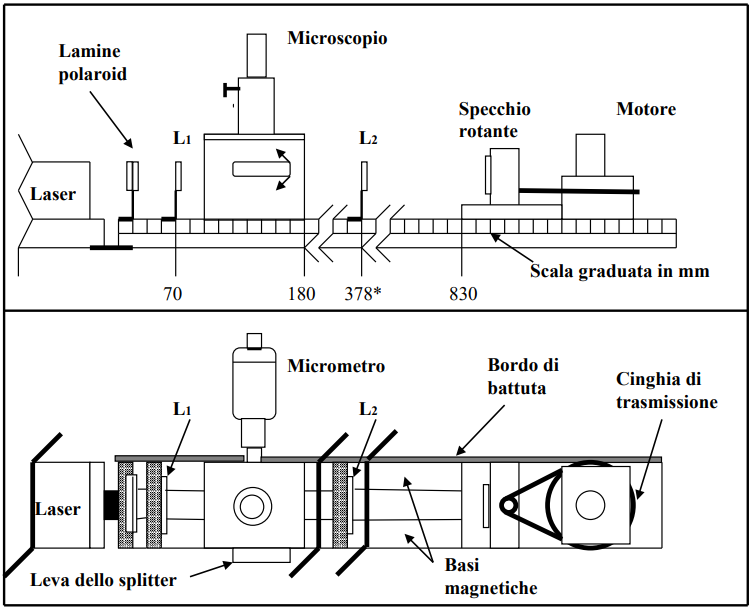
\includegraphics[scale=0.5]{Immagini/Apparato.png} 
  \centering
  \caption{Dalla seguente immagine si può visualizzare schematicamente l'apparato sperimentale in due prospettive: la vista laterale e dall'alto in modo da comprendere con maggiore dettaglio le varie componenti.}
  \label{Pro}
\end{figure}
Le lenti $L_1$, di distanza focale $f_1=48mm$, e $L_2$, di distanza focale $f_2=252mm$ (entrambe le misure note con un'incertezza $\sigma_f=1mm$) sono poste tra il laser e lo specchio rotante per garantire che la sorgente rimanga puntiforme durante tutta la distanza in quanto il laser, a lunghe distanze diventa un fascio di luce divergente. I supporti delle lenti sono dotati di magneti in grado di ancorarli con una certa stabilità alle basi magnetiche poste lungo il banco ottico. L'asse delle lenti può essere leggermente traslato poiché anche le lenti sono magneticamente attaccate ai loro supporti.

Tra le due lenti viene inserito un supporto che include lo splitter e il microscopio.
Lo splitter è una superficie di vetro semiargentata, orientata in modo da indirizzare il fascio luminoso di ritorno nel cannocchiale, posto in verticale perpendicolarmente al piano e al di sopra dello splitter. Per garantire ciò, la superficie semiriflettente deve essere la seconda ad essere attraversata dal raggio luminoso uscente dalla sorgente.

Sia il supporto delle lenti che dello splitter devono essere posizionati contro il bordo di battuta e durante l'esperienza occorre assicurarsi che non ruotino per evitare che si perda precisione nel posizionamento dei componenti.

Lo specchio rotante è collegato attraverso una cinghia di trasmissione ad un motorino, ed è regolabile la frequenza della sua rotazione mediante un dispositivo che presenta:
\begin{itemize}
    \item un interruttore di accensione (ON-OFF),
    \item un interruttore per la scelta del senso di rotazione (CW-CCW),
    \item una manopola per aumentare e diminuire gradualmente la frequenza di rotazione,
    \item un display che mostra la frequenza di rotazione,
    \item un pulsante che permette di portare la frequenza al massimo raggiungibile (circa 1500 giri al secondo) per un tempo massimo di 60 secondi,
    \item una luce rossa che indica un surriscaldamento o un problema del dispositivo e che invita a spegnere l'apparato se rimane acceso per più di 5 secondi.
    

\end{itemize}
Per allungare il più possibile la distanza D tra lo specchio rotante e lo specchio concavo, sono stati utilizzati gli specchi piani $S_1$ ed $S_2$ che permettono in uno spazio ridotto di raddoppiare le lunghezze in gioco. Per ultimo, Lo specchio concavo $M_f$ completa l'apparato sperimentale, riflettendo il raggio luminoso e dando origine al fascio di ritorno.
\begin{figure}[htp!]
  \centering
  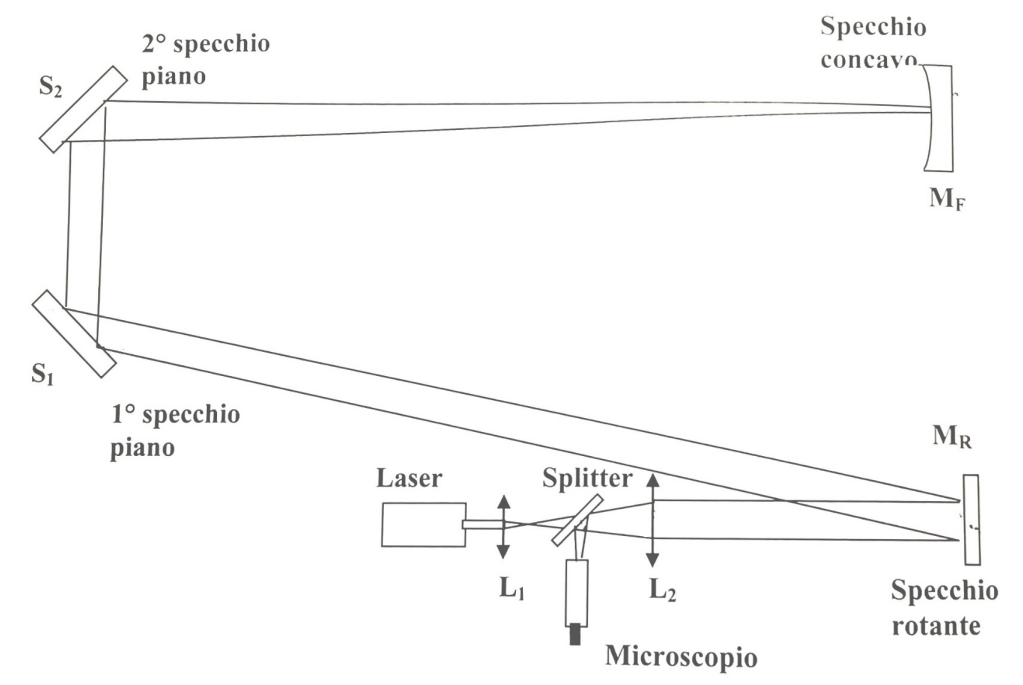
\includegraphics[scale=0.4]{Immagini/Apparato sperimentale.png} 
  \centering
  \caption{Nella seguente immagine si può osservare in modo schematico l'apparato sperimentale e il percorso che il fascio di luce laser compie durante l'esperimento.}
  \label{App}
\end{figure}


\subsection{Preparazione della strumentazione}
La prima parte dell'esperienza consiste nell'apportare degli aggiustamenti preliminari per preparare l'apparato sperimentale.
Dentro il laboratorio è già presente l'apparato che si può schematicamente osservare nell'immagine (\ref{App}). Per prima cosa bisogna misurare la distanza che il fascio di luce proveniente dalla sorgente laser compie durante il tragitto. Il laser infatti colpisce lo specchio rotante, arriva al primo specchio piano, viene riflesso nel secondo specchio piano ed infine arriva allo specchio concavo. Si può schematizzare questa distanza utilizzando le sorgenti immagini proveniente dalle varie riflessioni. Questa misura è la distanza $D$. Successivamente, con l'ausilio di una squadretta bianca, bisogna verificare che la luce laser sia allineata al centro dello specchio rotante con una tolleranza di $(1-2)\,mm$. \\


Dopodiché si inserisce la prima lente $L_1$ con lunghezza focale $f_1=48\,mm$ a $7 \,cm$ dalla sorgente assicurandosi che il fascio di luce non venga deviato e rimanga allineato con il centro dello specchio rotante. Dopo aver inserito la prima lente si inserisce il porta beam splitter a $18 \,cm$ dalla sorgente. Nel posizionare le lenti e il porta beam splitter bisogna sempre assicurarsi di seguire la guida metallica in modo da allineare tutte le ottiche e non propagare errori sistematici. In seguito si posiziona la lente $L_2$ con una lunghezza focale di $f_2=252\, mm$ ad una distanza di $37.8\,cm$ dalla sorgente. Analogamente al posizionamento della lente $L_1$ bisogna assicurarsi che il fascio di luce non sia stato deviato lungo il suo tragitto e sia ancora centrato nello specchio rotante. In caso contrario è possibile agire sul piano del supporto delle lenti ($L_1$ ed $L_2$) per modificare la direzione del fascio in quanto posizionate magneticamente sul proprio supporto. Una volta posizionate tutte le ottiche lungo la guida magnetica bisogna agire sulla cinghia di trasmissione per rendere la faccia piana dello specchio rotante perpendicolare al fascio di luce. In questo modo è possibile indirizzare il fascio di luce verso lo specchio $S_1$ e successivamente verso lo specchio $S_2$. Successivamente bisogna agire sulle viti presenti dietro gli specchi per modificare la loro inclinazione e indirizzare la riflessione del fascio di luce al centro dello specchio concavo.\\

Sulla superficie dello specchio concavo si forma un'immagine della sorgente la cui dimensione può essere modificata spostando la lente $L_2$ lungo la guida magnetica. L'obbiettivo è infatti ridurre al minimo la dimensione dell'immagine presente sullo specchio concavo in modo tale da individuare la posizione dell'immagine all'interno del microscopio con meno ambiguità. 
Per riuscire a misurare la posizione dell'immagine virtuale formata dallo specchio rotante all'interno del microscopio è necessario allineare i cammini di andata e di ritorno del fascio di luce. Con l'ausilio di una foglio di carta traslucida è possibile individuare entrambi i fasci di luce (di andata e di ritorno), ricordandosi che nel momento in cui si copre il fascio di luce di andata quello di ritorno smette di esistere (poiché la luce non raggiunge lo specchio concavo. Effettuando piccoli aggiustamenti alle viti dello specchio concavo e attraverso l'aiuto di un'altra persona che utilizza la carta traslucida per individuare la posizione del fascio di luce di ritorno rispetto al fascio di luce di andata bisogna allineare i due punti. Per farlo, si è verificata la posizione dei due fasci con la carta traslucida in tre diversi posizione lungo il tragitto: vicino allo specchio rotante, in una posizione intermedia tra i due specchi piani e lo specchio concavo ed infine vicino ai due specchi piani.\\

Successivamente, se sono stati eseguiti correttamente tutti gli aggiustamenti preliminari, posizionando la carta traslucida sopra il foro in cui va inserito il microscopio si dovrebbe vedere un punto luminoso. All'interno del microscopio è presente una griglia per agevolare la presa dati, per questo motivo è utile spostare il porta beam splitter fino a visualizzare il punto luminoso al centro del foro, in modo tale da allinearlo con la griglia.\\

Per questioni di sicurezza bisogna inserire sulla guida magnetica un filtro polarizzante tra il laser e la prima lente $L_2$ e successivamente si può montare il microscopio. Dopo aver acceso il motore responsabile della rotazione dello specchio e dopo aver impostato la frequenza di rotazione intorno ai $20-30 \, Hz$ si può togliere il filtro polarizzante e guardare all'interno del microscopio. All'interno si può visualizzare un punto luminoso che con l'aumentare della frequenza di rotazione dello specchio si sposta verso il basso o l'alto in base al senso di rotazione dello specchio.

\section{Procedura sperimentale}

\subsection{Metodo di raccolta dati}
Prima di preparare la strumentazione come spiegato nel paragrafo precedente, si è misurata la lunghezza $D$ come somma tra le le lunghezze $ \overline{M_rS_1}+\overline{S_1S_2}+\overline{S_1M_f}$. In particolare, per effettuare tale misura si è utilizzato un metro a nastro dotato di scala graduata con precisione $\sigma_{metro}=1\,cm$. Avendo a che fare con grandezze dell'ordine di metri, ed essendo il nastro morbido, è stato necessario assicurarsi che il nastro rimanesse diritto teso e non si inconcasse al centro. Per fare ciò, uno sperimentatore si è assicurato di tenere sollevata la parte centrale del nastro , evitando allo stesso tempo di modificarne la direzione e cercando di allineare il centro con le estremità.
In questo modo, la misura di $D$ e il suo errore sono state ricavate da
\begin{equation}
    D=\overline{M_rS_1}+\overline{S_1S_2}+\overline{S_1M_f} \, \, \, \, \, \, \, \, \, \, \, 
    \sigma_D=\sqrt{3\sigma_{metro}}=2cm
\end{equation}

Dopo aver sistemato le lenti come spiegato al paragrafo precedente, è stato possibile misurare la grandezza $a$, la distanza tra la seconda lente $L_2$ e lo specchio rotante, grazie al metro presente sul banco ottico, con la precisione di $\sigma_a=1mm$. 

Per le misure di $\Delta\delta$, si è utilizzato il microscopio, dotato di una una croce sulla lente e una rotella sul supporto indispensabili per centrare il punto luminoso corrispondente al raggio di ritorno. 

Una volta scelto il senso di rotazione dello specchio, è stato messo in moto con una frequenza bassa $\nu_0$ (intorno ai 50-100 Hz) e, ruotando appositamente la rotella, si è centrata con la croce del microscopio la posizione in cui appariva il punto luminoso del fascio di ritorno.  
Fatto ciò, si è trovata la misura $\delta_0$ leggendo la scala graduata posta sulla rotella (dotata anche di nonio, in grado di fornire misure con una precisione di 0.01mm)
Dopodiché, si è aumentata la frequenza a un valore $\nu$, si è riposizionato il mirino nel microscopio e si è trovata la misura $\delta_f$. 

Dalla formula (\ref{delta}) si ricava:
\begin{equation}
    c=\frac{4D^2b\omega}{\delta(D+a)}.
    \label{c}
\end{equation},
Sperimentalmente,ci si rende conto che la misura d $b$ risulta estremamente complessa in questo apparato: si sfrutta pertanto la legge dei punti coniugati, per cui si ha
\begin{equation}
    \frac{1}{b}+\frac{1}{D+a}=\frac{1}{f_2}
\end{equation}
dove tutti i valori tranne $b$ sono noti. Se ne ricava
\begin{equation}
    b=\frac{f_2(D+a)}{D+a-f_2}
\end{equation}
che può essere inserito all'interno della formula (\ref{c}) a ottenere:
\begin{equation}
    c=\frac{4f_2D^2(\omega)}{(D+a-f_2)\delta}.
    \label{c'}
\end{equation}
In particolare, risulta significativo partire ogni set di misure con una velocità angolare iniziale non nulla (per ridurre incertezze legate al meccanismo): si sfrutta dunque una simile formulazione delle formula (\ref{c'}) che tiene conto della rotazione iniziale:
\begin{equation}
    c=\frac{4f_2D^2(\omega_f-\omega_0)}{(D+a-f_2)\Delta\delta}
\end{equation}
dove $\omega_f$ e $\omega_0$ rappresentano le velocità angolari relative a $\nu_f$ e $\nu_0$ (si ricorda la legge $\omega=2\pi\nu$).

Una volta effettuate misure per rotazioni dello specchio sia in senso orario che in senso antiorario, è stata utilizzata la funzione di rotazione a massima frequenza e si sono effettuati molteplici misure considerando con $\nu_0$ la massima frequenza in un senso e con $\nu_f$ la massima frequenza nell'altro. In questo modo si è cercato di ottenere un $\Delta\delta$ molto grande.
\subsection{Analisi degli errori}
Analizzando l'incertezza sulle misure della velocità della luce $c$, si ritrovano due diverse categorie di errori che la generano:
\begin{itemize}
    \item errore sistematico, dovuto all'incertezza sulle misure $D$, $a$ ed $f_2$. Mediante il metodo della propagazione degli errori, si può calcolare $\sigma_{sis}$.
    Tale quantità corrisponde ad una incertezza presente in tutte le misure, che non può essere ridotta utilizzando metodi statistici.
    
    \item errore casuale, dovuto all'incertezza presente sulle misure $\Delta\delta$ e $\Delta\omega$, che variano di misura in misura. In particolare, l'incertezza che caratterizza la misura di $\Delta\delta$ è molto significativa, poiché con uno strumento dotato di precisione $0.01mm$ si misurano distanza comprese tra $0. 05mm $ e $1mm$ (ovviamente tale criticità risulta meno importante nel caso del turbo).
    L'incertezza sulla misura della velocità dovuta all'errore casuale può essere ridotta usando strumenti statistici, in particolare la deviazione standard della media, data dalla formula:
    \begin{equation}
         \sigma_{\bar{c}}=\sqrt{\frac{\sum_{i=1}^{n} (c_i-\bar{c})^2}{N(N-1)}}
    \end{equation}
\end{itemize}

L'incertezza totale sulla misura finale di $c$ è dunque dato da
\begin{equation}
    \sigma_c=\sqrt{\sigma_{\bar{c}}^2+\sigma_{sis}^2}
\end{equation}

In particolare si ricaveranno le misure di c per i tre differenti metodi di sperimentazione (rotazione dello specchio in senso orario, in senso antiorario e usando il turbo nei due sensi), in modo da assicurarsi che le misure in ogni set di dati siano ottenute con procedure e strumentazioni uguali.
\section{Analisi dei dati}
Le prime misure effettuate in laboratorio sono state le varie distanze che compie il fascio di luce laser. 
Le lunghezze delle misure $\overline{M_rS_1}$, $\overline{S_1S_2}$ e $\overline{S_1M_f}$ sono riportate nella tabella sottostante (\ref{parziali di D}):
 \begin{table}[ht]
    \centering
    \begin{tabular}{|c|c|c|}
    \hline
     $\overline{M_rS_1}$ [m] & $\overline{S_1S_2}$ [m] & $\overline{S_1M_f}$ [m]\\
    \hline
    $6.06 \pm\, 0.01$ & $0.66 \pm\, 0.01$ & $6.60 \pm\, 0.01$ \\
    \hline
    \end{tabular}
    \caption{In questa tabella sono riportate le lunghezze delle varie componenti che costituiscono il tragitto del fascio dallo specchio rotante allo specchio concavo }
    \label{parziali di D}
\end{table}




Nella tabella sottostante (\ref{primidati}) la grandezza $f_2$ rappresenta la distanza focale della lente $L_2$, la grandezza $D$ rappresenta la distanza tra lo specchio rotante e lo specchio concavo, la grandezza $a$ rappresenta la distanza tra la lente $L_2$ e lo specchio rotante.
\begin{table}[ht]
    \centering
    \begin{tabular}{|c|c|c|}
    \hline
     $f_2$[m] & $D$ [m] & $a$[m] \\
    \hline
    $0.252\pm0.001$ & $13.32\pm0.02$ & $0.451\pm0.001$ \\
    \hline
    \end{tabular}
    \caption{In questa tabella sono riportate le misure preliminari effettuate in laboratorio sull'apparato con le relative incertezze: $f_2$ è la lunghezza focale della lente $L_2$, $D$ è la distanza tra lo specchio rotante e lo specchio concavo e $a$ è la distanza tra la lente $L_2$ e lo specchio rotante.}
    \label{primidati}
\end{table}
\subsection{Senso antiorario}
Il primo set di misure prese sono state effettuate facendo girare lo specchio in senso antiorario:
\begin{table}[ht]
    \centering
    \begin{tabular}{|c|c|c|c|c|}
    \hline
     $\nu_0$ [$Hz$] & $\nu$ [$Hz$] & $\Delta \omega$ [1/s] & $\Delta\delta[m]$ & $c_{spe}$ [$m/s$] \\
    \hline
    $105$ & $282$ & $1112.12$ & $4\times10^{-5}$ & $3.678\times10^8$ \\
    \hline
    $643$ & $860$ & $1363.45$ & $7\times10^{-5}$ & $2.577\times10^8$ \\
    \hline
    $271$ & $426$ & $973.89$ & $4\times10^{-5}$ & $3.221\times10^8$ \\
    \hline
    $123$ & $522$ & $2506.99$ & $1.2\times10^{-4}$ & $2.764\times10^8$ \\
    \hline
    $522$ & $906$ & $2412.74$ & $1.2\times10^{-4}$ & $2.659\times10^8$ \\
    \hline
    $906$ & $1004$ & $615.75$ & $3\times10^{-5}$ & $2.715\times10^8$ \\
    \hline
    $69$ & $336$ & $1677.611$ & $7\times10^{-5}$ & $3.171\times10^8$ \\
    \hline
    $336$ & $611$ & $1727.88$ & $7\times10^{-5}$ & $3.265\times10^8$ \\
    \hline
    $611$ & $886$ & $1727.87$ & $8\times10^{-5}$ & $2.857\times10^8$ \\
    \hline
    $1004$ & $778$ & $1419.99$ & $6\times10^{-5}$ & $3.131\times10^8$ \\
    \hline
    $778$ & $482$ & $1859.82$ & $8\times10^{-5}$ & $3.075\times10^8$ \\
    \hline
    $1014$ & $735$ & $1753.01$ & $7\times10^{-5}$ & $3.313\times10^8$ \\
    \hline
    $735$ & $432$ & $1903.81$ & $1\times10^{-4}$ & $2.519\times10^8$ \\
    \hline
    $150$ & $897$ & $4693.54$ & $2.1\times10^{-4}$ & $2.957\times10^8$ \\
    \hline
    $817$ & $353$ & $2915.39$ & $1.30\times10^{-4}$ & $2.967\times10^8$ \\
    \hline
    $817$ & $431$ & $2425.31$ & $1\times10^{-4}$ & $3.208\times10^8$ \\
    \hline
    $431$ & $86$ & $2167.69$ & $1\times10^{-4}$ & $2.868\times10^8$ \\
    \hline
    \end{tabular}
    \caption{Tabella che contiene i dati effettuati facendo ruotare lo specchio in senso antiorario.}
    \label{antiorario}
\end{table}
Svolgendo la media tra le misure si ottiene:
\begin{equation}
    \nonumber
    c_{spe}=2.997\times10^8 \, \frac{m}{s} \qquad \sigma_c=7.8\times10^6 \, \frac{m}{s} 
\end{equation}
Per valutare quantitativamente la misura ottenuta rispetto al valore teorico di $c$ che nell'aria equivale a circa: $c_{teo}=2.998\times10^{8} \,ms^{-1}$ è stato effettuato il test t di Student con $N-1$ gradi di libertà dove $N$ è il numero che corrisponde alle misure effettuate:
\begin{equation}
    t=\frac{|c_{spe}-c_{teo}|}{\sigma_c}=0.015
\end{equation}
Dopo aver consultato le opportune tabelle si ottiene che c'è $98\%$ di probabilità che la misura sia diversa dal valore teorico per fluttuazioni statistiche.
\newpage
\subsection{Modalità turbo}
Successivamente, abbiamo preso un secondo set di dati con il "turbo". Questo metodo consiste nel sfruttare una modalità del motore dello specchio rotante che permetteva di raggiungere alte frequenze di rotazioni se pur in un breve periodo di tempo, dovuti al surriscaldamento. Di seguito sono presenti tutti i dati presi utilizzando questo secondo metodo.
\begin{table}[ht]
    \centering
    \begin{tabular}{|c|c|c|c|c|}
    \hline
     $\nu_0$ [$Hz$] & $\nu$ [$Hz$] & $\Delta \omega$ [1/s] & $\Delta\delta[m]$ & $c_{spe}$ [$m/s$] \\
    \hline
    $1409$ & $-1487$ & $18705.04$ & $8.8\times10^{-4}$ & $2.812\times10^8$ \\
    \hline
    $1492$ & $-1497$ & $18780.44$ & $8.9\times10^{-4}$ & $2.792\times10^8$ \\
    \hline
    $1496$ & $-1508$ & $18874.69$ & $8.55\times10^{-4}$ & $2.920\times10^8$ \\
    \hline
    $1480$ & $-1493$ & $18679.91$ & $7.4\times10^{-4}$ & $3.339\times10^8$ \\
    \hline
    $1500$ & $-1523$ & $18994.07$ & $8.1\times10^{-4}$ & $3.102\times10^8$ \\
    \hline
    $1512$ & $-1509$ & $18981.50$ & $8.6\times10^{-4}$ & $2.919\times10^8$ \\
    \hline
    $1513$ & $-1500$ & $18931.24$ & $7.5\times10^{-4}$ & $3.339\times10^8$ \\
    \hline
    $1525$ & $-1518$ & $19119.73$ & $8.6\times10^{-4}$ & $2.941\times10^8$ \\
    \hline
    $1523$ & $-1504$ & $19019.20$ & $8\times10^{-4}$ & $3.145\times10^8$ \\
    \hline
    $1531$ & $-1510$ & $19107.17$ & $8.4\times10^{-4}$ & $3.009\times10^8$ \\
    \hline
    $1527$ & $-1498$ & $19006.64$ & $8.3\times10^{-4}$ & $3.029\times10^8$ \\
    \hline
    $1514$ & $-1506$ & $18975.22$ & $8.9\times10^{-4}$ & $2.821\times10^8$ \\
    \hline
    $1535$ & $-1508$ & $19119.73$ & $8.5\times10^{-4}$ & $2.976\times10^8$ \\
    \hline
    $1525$ & $-1504$ & $19031.77$ & $8.5\times10^{-4}$ & $2.962\times10^8$ \\
    \hline
    $1516$ & $-1513$ & $19031.77$ & $8.4\times10^{-4}$ & $2.997\times10^8$ \\
    \hline
    $1531$ & $-1513$ & $19126.02$ & $8.4\times10^{-4}$ & $3.012\times10^8$ \\
    \hline
    $1532$ & $-1514$ & $19138.58$ & $8.5\times10^{-4}$ & $2.979\times10^8$ \\
    \hline
    $1538$ & $-1527$ & $19257.96$ & $8.4\times10^{-4}$ & $3.033\times10^8$ \\
    \hline
    \end{tabular}
    \caption{Tabella che contiene i dati effettuati facendo ruotare lo specchio in modalità turbo.}
    \label{turbo}
\end{table}\\
Attraverso l'analisi dati già illustrata si ottiene:
\begin{equation}
    \nonumber
    c_{spe}=3.007\times10^8 \, \frac{m}{s} \qquad \sigma_c=4.3\times10^6\, \frac{m}{s}
\end{equation}
Si può ora verificare la consistenza del valore ottenuto con il valore teorico attraverso l'analogo test di compatibilità t di Student ottenendo con $17$ gradi di libertà:
\begin{equation}
    t=\frac{|c_{spe}-c_{teo}|}{\sigma_c}=0.21
\end{equation}
La probabilità che la misura sperimentale sia diversa dal valore teorico per fluttuazioni statistiche è del $84\%$.
\subsection{Senso orario}
Durante la fase sperimentale abbiamo riscontrato diversi problemi legati alla strumentazione messa a disposizione. Prendendo i dati in senso orario il display presente sul macchinario che gestiva la frequenza di rotazione dello specchio, non segnalava la corretta frequenza quando si superavano i $400\, Hz$. Ci si è accorti di questo fenomeno poiché si riscontrava facilmente che ad un aumento della frequenza di rotazione (testimoniata anche da un rumore più intenso prodotto dal motorino), corrispondeva una diminuzione significativa della frequenza riportata dal display. \'E stato possibile prendere qualche dato ma essendo pochi non hanno nessuna coerenza statistica che permette lo studio o l'analisi dati. 
\subsection{Confronto tra i dati ottenuti}
\'E possibile confrontare i due valori ottenuti utilizzando nuovamente il test del t di Student. In particolare, per questo tipo di confronti si utilizza la formula
\begin{equation}
    t=\frac{|c_1-c_2|}{\sqrt{\sigma_{c_1}^2+\sigma_{c_2}^2}}
\end{equation}
dove $c_1$ e $c_2$ sono i valori ottenuti dalle due esperienze e $\sigma_{c_1}$ e $\sigma_{c_2}$ i relativi errori. Il numero dei gradi di libertà in tale contesto è pari a $gdl=N_1+N_2-2$, dove $N_1$ e $N_2$ sono i numeri di dati acquisiti da ciascuna delle due esperienze.
Si ha dunque t=0.11 con 33 gradi di libertà, che corrisponde ad una probabilità del 91\% che la differenza ottenuta tra i due valori abbia origine statistica.

\section{Conclusione}
L'esperienza descritta ha come scopo stabilire il valore della velocità della luce, grandezza fondamentale per lo studio della fisica sulla cui misura sono state fatte nei secoli numerose analisi. La genialità del metodo proposto da Foucault, e che è stato ricreato abbastanza fedelmente in laboratorio, sta nel fatto che non si cerca un valore della velocità in maniera classica (ovvero come rapporto tra una distanza percorsa e il tempo necessario per percorrerla, che richiederebbe o spazi enormi o capacità di percepire tempi molto piccoli), ma, sfruttando fenomeni ottici, si riesce a lavorare con grandezze più facilmente misurabili senza strumenti estremamente sofisticati.
L'esperienza si basa su un raggio laser che, colpendo uno specchio piano ruotante , viene indirizzato verso uno specchio concavo, che lo costringe a ritornare indietro seguendo il medesimo percorso d'andata. Nel frattempo, lo specchio rotante cambia posizione: il laser di ritorno, colpendo lo specchio rotante, non verrà mandato verso la sorgente, ma verrà leggermente deviato. Conoscendo la dimensione di questa deviazione e alcune costanti proprie dell'apparato sperimentale (come la velocità angolare di rotazione dello specchio), risulta possibile calcolare la velocità della luce.

Purtroppo, non è stato possibile eseguire l'esperienza nel caso di rotazione in senso orario dello specchio a causa di un malfunzionamento di uno strumento fondamentale: il sensore in grado di misurare e comunicare la frequenza di rotazione dello specchio. \'E risultato infatti che tale strumento non era in grado di funzionare in maniera esatta quando si superava una frequenza di 400 Hz, rendendo impossibile ottenere misure valide della velocità della luce.

Questo problema non si è manifestato invece per le rotazioni in senso antiorario, dove si sono registrati numerosi dati che hanno permesso di calcolare la velocità della luce $c$ come:
\begin{equation}
    c_{CCW}=(2.997\pm0.078)\times 10^8\frac{m}{s}.
\end{equation}
Questo valore è stato confrontato con la velocità reale $c=(2.9979\times 10^8)\frac{m}{s}$ mediante il confronto tramite t di Student, e si è registrato 98\% di probabilità che la differenza abbia avuto origine statistica.

\'E stato poi possibile sfruttare una funzionalità del motorino collegato allo specchio rotante che permetteva di raggiungere la massima frequenza in entrambe le direzioni di rotazione e confrontare la posizione del raggio laser di ritorno nei due casi. Grazie a tale set di dati si è trovato un secondo valore della velocità della luce, pari a 
\begin{equation}
    c_{turbo}=(3.007\pm0.043)\times 10^8 \frac{m}{s}.
\end{equation}
Confrontando nuovamente il valore ottenuto con il valore atteso mediante il test del t di Student, risulta che esiste l'84\% si probabilità che la differenza tra i due abbia origini statistiche.

In entrambi i casi, sia nella rotazione antioraria che nell'utilizzo del "turbo", si sono ottenuti valori statisticamente coerenti al valore atteso.



\appendix



\end{document}
